\documentclass[a4paper, 12pt]{report}

% Charset
\usepackage[utf8]{inputenc}
% Language
\usepackage[british]{babel}
% Font
\usepackage[default]{sourcesanspro}
\usepackage[T1]{fontenc}
\usepackage{titlesec, color}
\definecolor{gray75}{gray}{0.75}
\newcommand{\hsp}{\hspace{20pt}}
\usepackage{microtype}
% Color
\usepackage{xcolor}
% Graphics
\usepackage{graphicx}
\usepackage{fancyhdr}
\graphicspath{ {./img/} }
% Indexing
\usepackage{index}
\makeindex

\usepackage{blindtext}

\begin{document}
% Title page
\title{\Large{\textbf{The Bitcoin Lightning Network}}}
\author{Yannick Mawuena Rüfenacht}
\date{October 21, 2020\\Version 1.0.0}
\maketitle

% Quote
\begin{quote}
\vspace*{\fill}
\textit{``Lightning is a decentralized network using smart contract functionality in the blockchain to enable instant payments across a network of participants."}
\par\raggedleft--- \textup{Joseph Poon}
\vspace*{\fill}
\end{quote}

% Table of Contents
\tableofcontents
\listoffigures

% Formatting
\setlength{\parskip}{1em}
\setlength{\parindent}{0em}
\titleformat{\chapter}[hang]{\LARGE\bfseries}{\thechapter\hsp\textcolor{gray75}{|}\hsp}{0pt}{\LARGE\bfseries}
\titleformat{\section}[hang]{\large\bfseries}{\thesection\hsp\textcolor{gray75}{|}\hsp}{0pt}{\large\bfseries}

\widowpenalties 1 10000
\raggedbottom

\chapter{Introduction}
\par The aim of this paper is to shed light onto the mysterious inner workings of the Lightning Network. The Lightning Network builds upon the underlying technology of the blockchain. It uses the blockchain and Bitcoin smart contracts to create a secure network of participants which are able to perform transactions at high volume and speed. To be able to understand how the lightning network works or why it is even necessary, requires a basic understanding of the blockchain and Bitcoin.
\par This paper guides the reader through a list of steps that show how the lightning network is built, starting from the basics of a blockchain. Each step builds on top of the previous one. It is therefore recommended to read this paper in the right order.

\chapter{A Brief Overview of the Bitcoin Blockchain}
\par The way of ordinary banking systems usually goes as follows: The customer deposits his money on a bank account and when a payment is done, the bank either adds or subtracts the amount from his or her account. Or sometimes the customer withdraws some money from the ATM. The underlying concern hereby is that in each of those use cases there is always one centralized system involved which is in power of handling all the transactions. The inner workings of that system are strictly sealed to the outside, which has the capability to create trust issues. And this is where the idea of Bitcoin comes to the surface.

\section{The Idea of Bitcoin}
\par The main idea of Bitcoin is to remove the aspect of centralized control and to form a network of users where everyone is connected to everyone and the same rights apply to everyone.  

\begin{figure}[h]
	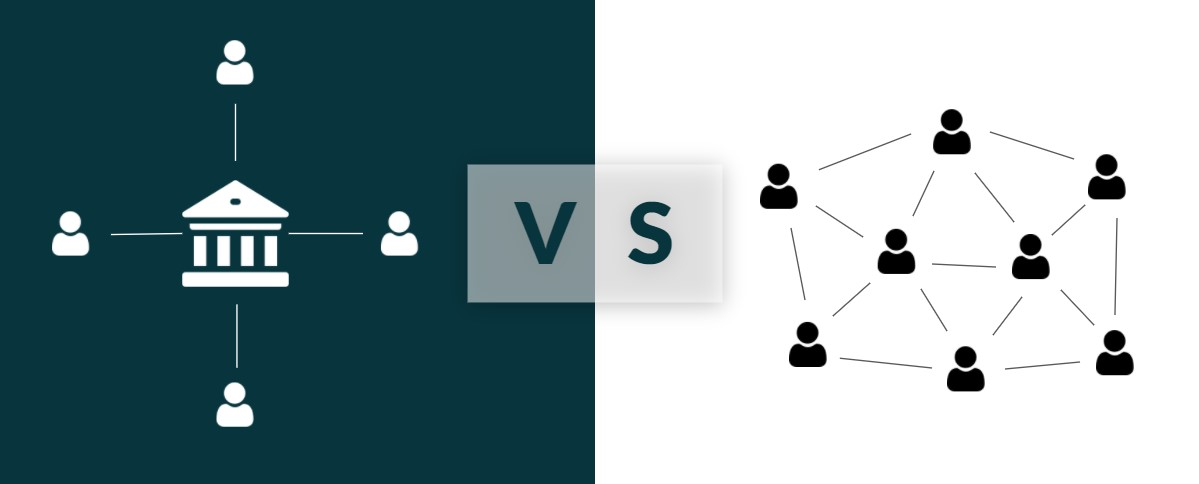
\includegraphics[width=\textwidth]{01_Decentralized}
	\caption{Conventional Banking System vs Decentralized System}
	\label{fig:01_Decentralized}
\end{figure}

\par To achieve this, the history of all transactions is stored in a public ledger, which is accessible to everyone. But instead of storing this ledger in one central place, every participant obtains their own copy so that the ledger is distributed to everyone throughout the network of participants. Anyone who then performs a transaction broadcasts it out to the entire world for everyone to hear and to include it in their private ledgers. 
\par At first, the degree of openness that this system provides might seem absurd. But the fact that all the records of the transactions are publicly available also means that everyone can verify the validity of every transaction. And this is where Bitcoin gains its immense trust and security benefits.

\section{The Issue of Decentralization}
\par Although the approach of a centralized network seems quite appealing so far, there is an important issue that arises very quickly. While the idea of everyone broadcasting their transactions to the entire network would work for a small number of people, it would become significantly more difficult to ensure that every member of the network receives every transaction in the same order, as the number of participants increases. Network delays could cause transactions to arrive in different orders in different places. This raises the question: How can the ledger maintain the right order of transactions across the entire network of participants. 
\par This is precisely the problem that was addressed in the original Bitcoin paper. The solution that Bitcoin offers lies within the functionality of its blockchain.

\section{The Bitcoin Blockchain}
\par In order to maintain the right order of all transactions, the broadcasting of new transactions needs to be regulated and a new mechanism that locks the order off all the transactions needs to be implemented.
\paragraph{Blocks} \hspace{0pt} \\
First of all, the ledger is split into a group of blocks. Each block contains a set of transactions and a special value at the bottom that is referred to as the “proof of work”. 

\begin{figure}[h]
	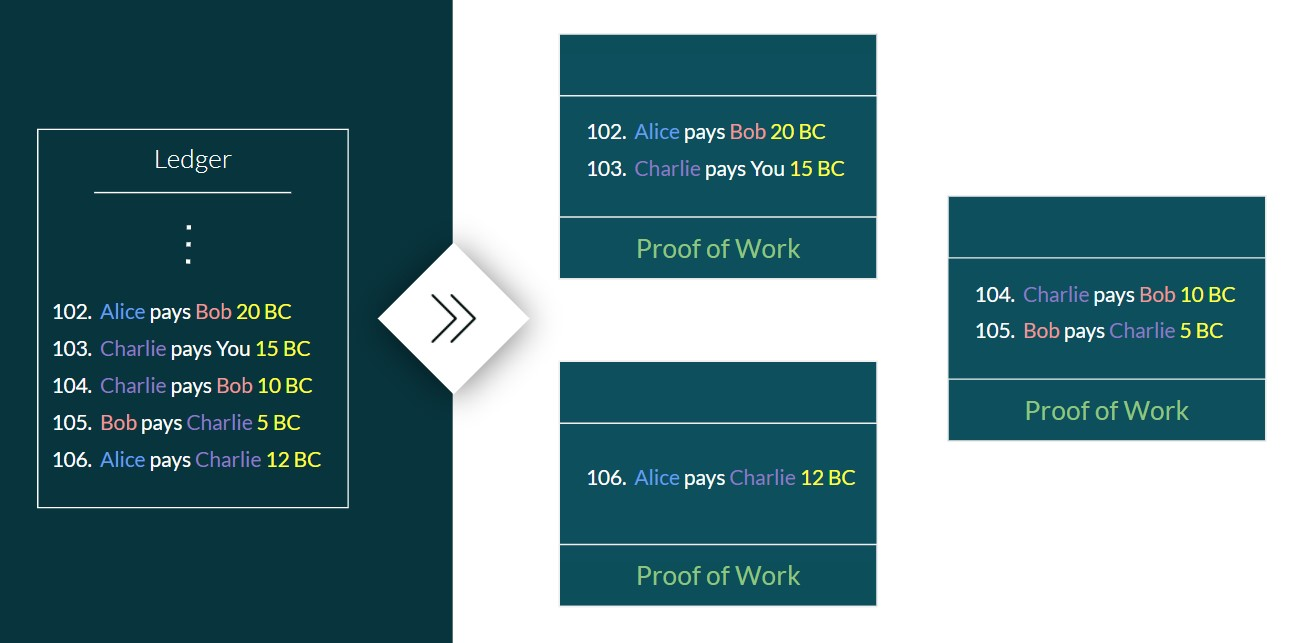
\includegraphics[width=\textwidth]{02_Ledger_Blocks}
	\caption{Ledger being split into blocks}
	\label{fig:02_Ledger_Blocks}
\end{figure}

\paragraph{Proof of work} \hspace{0pt} \\
The proof of work, also known as the hash of the block, is a special numeric value that is required for each block. A block without a proof of work is considered invalid. The value is special in the sense that it needs to be calculated. The calculation takes on average 10 minutes of computational work. This process is usually performed by special members of the network called “Minors”. The purpose of this mechanism is to regulate the number of transactions that are being broadcasted and to make it difficult for attackers to generate new blocks. Furthermore, the proof of work is unique for each block, this means that it could also act as a unique identifier.
\paragraph{Ordering transactions} \hspace{0pt} \\
To maintain a fixed order to these blocks, each block additionally contains the proof of work of its previous block.\footnote{The first block is a special case since it cannot point to a previous block. It is named the Genisis Block} This causes each block to have a reference to its previous block which ultimately results in a fixed list.

\begin{figure}[h]
	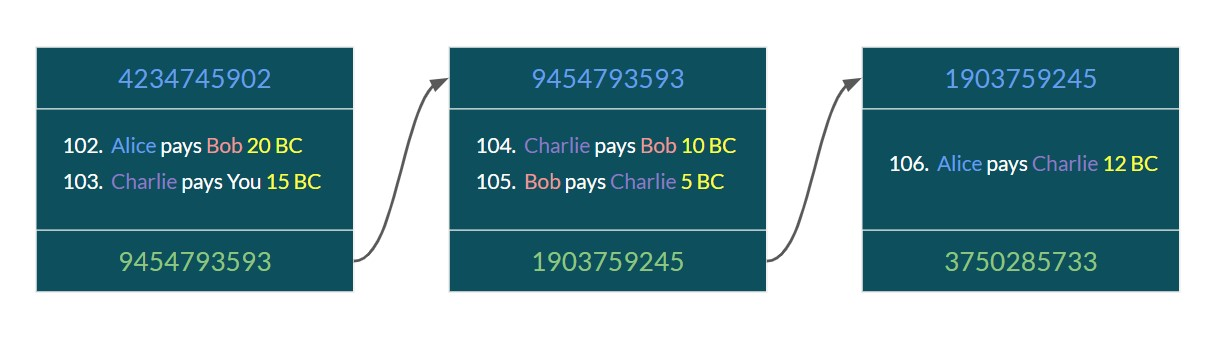
\includegraphics[width=\textwidth]{03_Linked_Blocks}
	\caption{Chaining of the blocks}
	\label{fig:03_Linked_Blocks}
\end{figure}

\paragraph{Security} \hspace{0pt} \\
The proof of work, or hash, is unique for each block as aforementioned. It is calculated using the contents of the block i.e., the set of transactions and the hash of the previous block. If the content gets changed, the hash automatically gets changed as well. The fact that each block contains the hash of the previous block is precisely what makes the blockchain so secure. 
\par If for example the content of the second block from the picture above gets tampered, it would automatically change its hash. This in turn would make the third block invalid since it no longer stores a valid hash of its previous block. Altering the third block causes the fourth block to be invalid. This scenario repeats itself throughout the entire list. This means that changing one block would consequently require changing the entire chain of blocks for it to be valid again. 
\par Since the ledger now basically consists of a group of blocks that are immutably chained together, it is commonly referred to as the “blockchain”. 

\section{The Ledger is the Currency}
\par Bitcoin is said to be a cryptocurrency. This poses the question: What actually is a cryptocurrency? The answer is quite simple: \textit{It is a ledger. The history of transactions is the currency.}
\par That being said, it is theoretically possible to remove the need for cash. Hypothetically, if everyone in the world used this ledger, it would be possible to send and receive money on this ledger for all eternity without ever converting it to cash.

\chapter{The Scalability Problem with Bitcoin}
\par As far as safety is concerned, Bitcoin does an excellent job with its use of distributed ledgers. However, as a payment platform, Bitcoin by itself cannot handle the whole transactions of the world anytime in the near future.

\chapter{Introducing the Lightning Network}
\section{Multi-Signatures}
\section{Timelocks}
\section{Micropayment Channels}
\section{Bi-directional Payment Channels}
\section{Hash and Timelock Contracts}
\section{Routing}

\chapter{Protential Risks of the Lightning Network}
\section{Coin Theft via Tracking}

\chapter{Use Cases}
\section{Instant Payment in a Coffee Shop}
\section{Micropayments for Internet Service}
\section{Routed Payments}

\end{document}
